\documentclass{article}
\usepackage{spconf,amsmath,epsfig}
\usepackage{booktabs}
\usepackage{oldstyle}
\usepackage{subfigure}
\usepackage{hyperref}

\graphicspath{{../figures/}{../figures/generated/}{../images/}}

\title{Nuclear Segmentation in Microscope Cell Images: A Hand-segmented Dataset and Comparison of Algorithms}
\name{Lu\'\i s Pedro Coelho$^{1,2,3}$, Aabid Shariff~$^{1,2,3}$, Robert F.\ Murphy$^{1,2,3,4,5}$}
\address{$^1$Lane Center for Computational Biology, Carnegie Mellon University\\
        $^2$Center for Bioimage Informatics, Carnegie Mellon University\\
        $^3$Joint Carnegie Mellon University--University of Pittsburgh PhD.\ Program in Computational Biology\\
        $^4$Depts.\ of Biological Sciences, Biomedical Engineering, and Machine Learning, Carnegie Mellon University\\
        $^5$External Fellow, Freiburg Institute for Advanced Studies, University of Freiburg, Germany}
%
% For example:
% ------------
%\address{School\\
%	Department\\
%	Address}
%
% Two addresses (uncomment and modify for two-address case).
% ----------------------------------------------------------
%\twoauthors
%  {A. Author-one, B. Author-two\sthanks{Thanks to XYZ agency for funding.}}
%	{School A-B\\
%	Department A-B\\
%	Address A-B}
%  {C. Author-three, D. Author-four\sthanks{The fourth author performed the work
%	while at ...}}
%	{School C-D\\
%	Department C-D\\
%	Address C-D}
%
\newcommand*{\indicator}[1]{\hspace{1pt}[\hspace{-.4em}[\hspace{3pt} #1 \hspace{3pt}]\hspace{-.4em}]\hspace{2pt}}
\newcommand*{\ttt}{\textsc{nih}{\footnotesize 3}\textsc{t}{\footnotesize 3}}
\newcommand*{\utos}{\textsc{u{\footnotesize 2}os}}
\bibliographystyle{IEEEbib}
\begin{document}
\maketitle
%
\begin{abstract}
Image segmentation is an essential step in many image analysis pipelines and many algorithms have been proposed to solve this problem. However, they are often evaluated subjectively or based on a small number of examples. To fill this gap, we hand-segmented a set of 97~fluorescence microscopy images (a total of 4009~cells) and objectively evaluated some previously proposed segmentation algorithms.

We focus on algorithms appropriate for high-throughput settings, where only minimal user intervention is feasible.

The hand-labeled dataset (and all software used to compare methods) is publicly available to enable others to use it as a benchmark for newly proposed algorithms.
\end{abstract}
%
\begin{keywords}
Biomedical image processing, Image segmentation
\end{keywords}
%
\section{Introduction}\label{sec:intro}

Nuclear segmentation is an important step in the pipeline of many cytometric analyses. It forms the basis of many simple operations (cell counting, cell-cycle assignment,\ldots) and is often the first step in cell segmentation. However, algorithms are often evaluated subjectively or based on a few examples. In order to objectively evaluate nuclear segmentation algorithms, we built a dataset of hand-segmented fluorescence microscopy images.

We also evaluated some published algorithms for this problem on our hand-labeled dataset. We were interested in algorithms that were applicable to large-scale automated data collection. Therefore, while parameter tuning for the properties of a given image collection was an acceptable burden on the human operator, tuning for single images was not.

Bamford ~\cite{Bamford2003Empirical} undertook a similar effort in bright-field microscopy images of cell nuclei.  Recently, Gelasca et al.~\cite{Gelasca08-298} made a available a series of ground truth assignments for different tasks in bioimage segmentation, but it did not include a dataset of hand-labeled single nuclei. Our dataset is thus a complement to their work.

\section{Dataset}\label{sec:format}

The dataset is composed of two different collections (Table~\ref{tab:dataset}). The first collection is of \utos{} cells, originally created for a study of pattern unmixing algorithms~\cite{TaoBonami}. Figure~\ref{fig:gnf-examples} shows two images from this collection. An initial set of 50~images from this collection was chosen, but 2~images were rejected as containing no in-focus cells.

\begin{table}
\centering
\begin{tabular}{lrr}
\toprule
& \utos{} & \ttt{} \\
\midrule
Pixel size           & $1349 \times 1030$ & $1344 \times 1024$ \\
Nr.\ Cells           &  1831              &  2178              \\
Avg.\ Cover          &   23\%             &    18\%            \\
Min Nr.\ Cells       &   24               &    29              \\
Max Nr.\ Cells       &   63               &    70              \\
\bottomrule
\end{tabular}
\caption{Main Properties of the Two Collections. Avg.\ cover denotes the percentage of pixels covered by cells. The minimum and maximum are over all the images in each collection.}
\label{tab:dataset}
\end{table}

\begin{figure*}
\begin{center}
\subfigure[``Easy'' image]{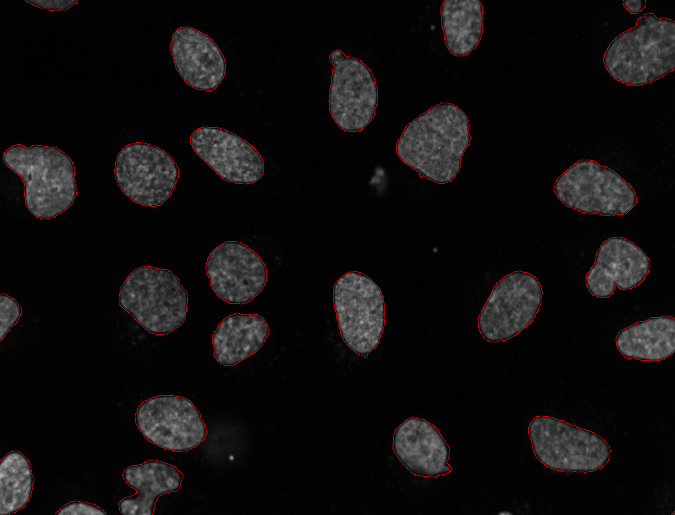
\includegraphics[width=.43\textwidth]{gnf-segmented-4}}\quad
\subfigure[``Difficult'' image]{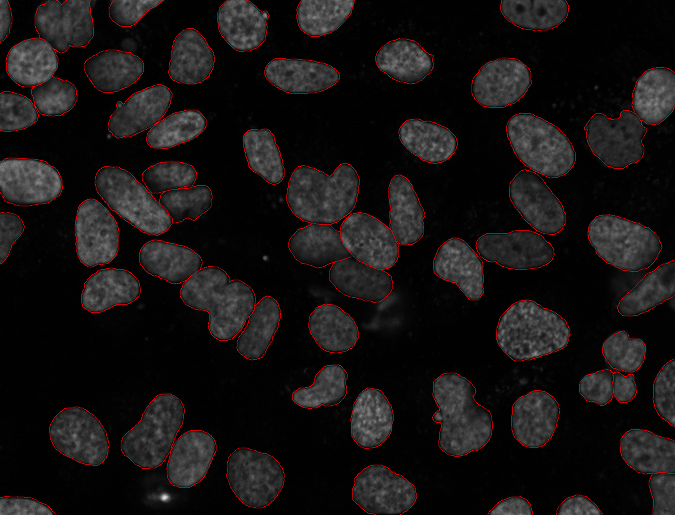
\includegraphics[width=.43\textwidth]{gnf-segmented-41}}
\end{center}%
\caption{Two example images from the \utos{} collection. (a) shows nuclei that are well separated. Automatic segmentation is expected to do well. (b)  has many clustered nuclei and is expected to challenge segmentation algorithms. Most images in the collection lie in between these two examples.}%
\label{fig:gnf-examples}%
\end{figure*}
The second collection is of \ttt{} cells, collected using the methodology reported by Osuna et al.~\cite{GarciaOsuna2007}. Nuclei in this group are further apart and there is less clustering. They are also more homogeneous in shape and size (data not shown). On the other hand, nuclei in single images vary greatly in brightness and images often contain visible debris. Therefore, we consider this a more challenging dataset for automated methods. Fifty images were initially chosen, but one was rejected as containing no in-focus cells.

Manual segmentation was performed by outlining nuclei with a computer mouse. Only the nuclear marker image was used for this process. All images were segmented by one of the authors (L.P.C.) and a subset of 10~images (5 from each collection) were independently segmented by another (A.S.).  

The hand-labeled dataset and all software necessary to generate the results in this paper are available at \linebreak\href{http://murphylab.web.cmu.edu/data}{http://murphylab.web.cmu.edu/data} and \linebreak\href{http://murphylab.web.cmu.edu/software}{http://murphylab.web.cmu.edu/software}.

\section{Methods}\label{sec:method}

\subsection{Segmentation}

Due to space limitations, we will only describe the ways in which our implementation was adapted to our images and refer the reader to the original publications for detail.

\subsubsection{Thresholding}

We considered 3~thresholding methods: Ridler-Calvard~\cite{RCthresh}, Otsu~\cite{otsu_ieeetsmc_1979}, and mean pixel value. All above-threshold contiguous regions are considered objects. To remove some noise, we filter the thresholded image with a median filter (window of size~5).

To remove small non-nuclear objects, we filter out objects smaller than 2500~pixels, circa 64~square microns. This post-filtering was applied to all segmentation results in this paper.

\subsubsection{Seeded watershed}

We implemented two versions of seeded watershed, both run on a thresholded version of the image (using the mean as threshold, which, as we show below, is the better thresholding method for these images). One operates directly on a blurred version of the image\footnote{We used a gaussian blur with a width of 12~pixels.}, while the second one operates on the gradient of the image. In both cases, seeds are regional maxima of the blurred image.

\subsubsection{Active masks}

Active masks are a recent proposal by Srinivasa et al.~\cite{DBLP:conf/isbi/SrinivasaFGHGLK08}. The algorithm assumes that there are two classes of objects, foreground and background. Its only parameters are the mean value and standard deviation of the background region.\footnote{The active mask framework is more general than this, but we restrict ourselves to the original proposal.}

Manual tuning led to the following semi-automatic procedure for parameter setting: the value of the background mean is assumed to be the histogram peak plus~3, while the background standard deviation is set to~0.5.

\subsubsection{Merging Algorithm}

Lin et al.~\cite{LinRoysam} described an algorithm that is based on merging multiple regions obtained from watershed segmentation, using shape information learned from a labeled dataset. We have implemented a slight variation of their algorithm, but retained the structure. In particular, we use the mean method for segmentation, and as shape features: fraction of area that is contained in the convex hull, roundness, eccentricity, area, perimeter, semi-major, and semi-minor axes (all, except the first, computed on the convex hull). Apart from these minor changes, the algorithm is unchanged.

For the studies below, the set segmented by A.S.\ was used for training and the set segmented by L.P.C.\ (except the images that are common to both segmentations) were used for testing.

\subsection{Evaluation}

Several metrics have been proposed for evaluation of segmentation results against a hand-labeled standard. Some approaches stem from viewing segmentation as a form of clustering of pixels. This allows the use of metrics developed for the evaluation of clustering results. From this family of approaches, we used the Rand and Jaccard indices~\cite{RandDec1971,Saporta02comparingtwo}.

The disadvantage of such metrics is that they do not take into account the spatial characteristics of segmentation. In fact, the exact location of the border between foreground and background is often fuzzy. An algorithm that returns a nucleus which almost matches the gold-standard except for a one-pixel-wide sliver around the border should be judged very highly even if that sliver contains a large number of pixels. Previous work on evaluation of bright-field microscopy images by Bamford~\cite{Bamford2003Empirical} used the Hausdorff metric.

\subsubsection{The Rand and Jaccard Indices}

Let $S$ be a (binary) segmented image and $R$ be a (binary) reference image. Let $i$ and~$j$ range over all pairs of pixels where $i \ne j$, then each pair falls into one of four categories: (a) $R_i = R_j$ and $S_i = S_j$, (b) $R_i \ne R_j$ and $S_i = S_j$, (c) $R_i = R_j$ and $S_i \ne S_j$, (d) $R_i \ne R_j$ and $S_i \ne S_j$. If we let $a,b,c,d$ refer to the number of pairs in its corresponding category, then the Rand~index is defined as:
\begin{equation}
\text{RI}(R,S) = \frac{a+d}{a+b+c+d}.
\label{eq:rand}
\end{equation}%
%
That is, the Rand index measures the fraction of the pairs where the two clusterings agree. The Rand index ranges from 0 to~1, with 1 corresponding to perfect agreement.

Based on the same definitions for $a,b,c,d$, the Jaccard index is defined as:
%
\begin{equation}
\text{JI}(R,S) = \frac{a+d}{b+c+d}.
\label{eq:jaccard}
\end{equation}%
The Jaccard index is not upper-bounded, but higher values correspond to better agreement.

\subsubsection{Error Counting}
Each object in the segmented image is assigned to the object in the reference image with which it shares the most pixels. Based on these assignments, we can define the following classes of errors: \textbf{split}: two segmented nuclei are assigned to a single reference nucleus; \textbf{merged}: two reference nuclei are assigned to a single segmented nucleus; \textbf{added}: a segmented nucleus is assigned to the reference background; and \textbf{missing}: a reference nucleus is assigned to the segmented background.

\subsubsection{Spatially-Aware Evaluation Methods}

We implemented two spatially-aware evaluation metrics. Both are based on assigning segmented nuclei to reference nuclei as above, as they are computed between pairs of matched objects. 

For each pixel, we compute its distance to the reference border. The normalised sum of distances is then defined as:
%
\begin{equation}
\text{NSD}(R,S) = \frac{\sum_{i}^{} \indicator{R_i \ne S_i}*D(i)} {\sum_{i}^{} D(i)},
\label{eq:nd}
\end{equation}%
where the sum index $i$ ranges over pixels in the union of both objects and $D(i)$ is the distance of pixel $i$ to the border of the reference object. From the equation, it is obvious that $\text{NSD}(R,S) \in [0,1]$, with $0$ corresponding to perfect agreement and $1$ to no-overlap. We note that the sum of distances is \emph{not} a metric as it is neither symmetric nor does it satisfy the triangle inequality. 

The Hausdorff metric is computed as described by Bamford~\cite{Bamford2003Empirical}. In the notation above it can be defined as:
%
\begin{equation}
H(R,S) = \max \left\{ D(i) : S_i \ne R_i \right\}.
\end{equation}
\section{Results}\label{sec:results}

\begin{table*}
\centering
\begin{tabular}{lcccccccccccc}
\toprule
Algorithm              & $\text{RI}$ & $\text{JI}$ & Hausdorff     & NSD ($\times 10$)          &   Split      & Merged      &   Spurious    & Missing     \\
\midrule                                                                                                                                   
AS Manual                & 95\%/93\%    & 2.4/3.4         & 9.7/12.0        & 0.5/0.7         & 1.6/1.0         & 1.0/1.2         & 0.8/0.0         & 2.2/3.2         & \\
RC Threshold             & 92\%/77\%    & 2.2/2.1         & 34.8/26.4       & 1.2/2.6         & 1.1/1.0         & 2.4/2.4         & 0.3/1.9         & 5.5/22.1        & \\
Otsu Threshold           & 92\%/74\%    & 2.2/2.1         & 34.9/36.7       & 1.2/3.5         & 1.1/0.8         & 2.4/2.1         & 0.3/1.7         & 5.6/26.6        & \\
Mean Threshold           & 96\%/82\%    & 2.2/1.9         & 26.5/24.4       & 1.0/2.3         & 1.3/1.4         & 3.4/5.1         & 0.9/3.1         & 3.6/4.8         & \\
Watershed (direct)       & 91\%/78\%    & 1.9/1.6         & 34.9/19.3       & 3.6/3.7         & 13.8/2.9        & 1.2/2.4         & 2.0/11.6        & 3.0/5.5         & \\
Watershed (gradient)     & 90\%/78\%    & 1.8/1.6         & 34.6/21.7       & 3.0/3.8         & 7.7/2.6         & 2.0/3.0         & 2.0/11.4        & 2.9/5.4         & \\
Active Masks             & 87\%/72\%    & 2.1/2.0         & 148.3/98.0      & 5.5/5.0         & 10.5/1.9        & 2.1/1.5         & 0.4/3.9         & 10.8/31.1       & \\
Merging Algorithm        & 96\%/83\%    & 2.2/1.9         & 12.9/15.9       & 0.7/2.5         & 1.8/1.6         & 2.1/3.0         & 1.0/6.8         & 3.3/5.9         & \\

\bottomrule
\end{tabular}
\caption{Comparison of Segmentation Algorithms. Result of various segmentation approaches are compared against the hand-segmented standard. Each entry contains two values corresponding to the statistic for two datasets used, \utos{} and \ttt{}, respectively.}
\label{tab:comparison}
\end{table*}

Table~\ref{tab:comparison} summarises the results obtained.

Both manual segmentations are in general agreement. Disagreements can be tracked down to an image where the authors differed on whether some small bright objects should be marked as nuclei or debris.

Both Otsu and Ridler-Calvard thresholding score poorly, missing many cells, particularly in the \ttt{} collection. In this collection, the presence of very bright cells leads the algorithm to set a threshold between the very bright cells and the rest of the cells, instead of setting it between the foreground and background. The mean thresholding is better suited for these images, which consist mainly of background with objects of very different intensities.

Watershed results in less merges than mean-based segmentation, but more split nuclei and spurious objects. Active masks score poorly mainly due to nuclei over-segmentation and missing objects. Lin et al.'s merging algorithm obtains very good results, dominating other algorithms in almost all metrics.

We also notice the Rand and Jaccard indices while distinguishing the alternative manual segmentation from the automatic ones are not good measures for this data as they fail to distinguish between the better and the worse algorithms. Both the Hausdorff and the NSD measures capture the relationships between the algorithms well.

\section{Discussion}\label{sec:discussion}

We presented a dataset that can be used to evaluate nuclear segmentation algorithms. This dataset consists of two collections, from different cell types and different microscopes.

We also implemented several published algorithms for nuclear segmentation and tested them against our standard.  The approach of Lin et al.~\cite{LinRoysam} emerged as the best scoring in most tests. We also concluded that the Hausdorff metric and the normalised sum of distances measure we propose captured the quality of the algorithms better than the alternatives under consideration.

\subsection{Acknowledgements}

This work was supported in part by NIH grants GM75205 and NSF ITR  grant EF-0331657 (R.F.M.). L.P.C.\ was partially funded by the Funda\c c\~ao Para a Ci\^encia e Tecnologia (grant SFRH/BD/37535/2007) as well as a fellowship from the Fulbright Program.

\bibliography{references}

\end{document}
